% ==============================================================================
% A Large-Scale Computational Study of Most Delayed Palindromic Numbers
% in the Reverse-and-Add Process
% ==============================================================================
\documentclass[11pt,a4paper]{article}

% --- Packages ---
\usepackage[margin=1in]{geometry}
\usepackage{amsmath,amssymb,amsfonts}
\usepackage{algorithm}
\usepackage{algorithmic}
\usepackage{booktabs}
\usepackage{hyperref}
\usepackage[round]{natbib}
\usepackage{pgfplots}
\pgfplotsset{compat=1.18}
\usepackage{tikz}
\usetikzlibrary{arrows.meta,positioning,shapes.geometric,calc,fit,backgrounds}
\usepackage{subcaption}
\usepackage{multirow}
\usepackage{xcolor}
\usepackage{graphicx}
\usepackage{enumitem}
\usepackage{microtype}

% --- Color definitions ---
\definecolor{recordblue}{RGB}{31,119,180}
\definecolor{searchorange}{RGB}{255,127,14}
\definecolor{fitgreen}{RGB}{44,160,44}
\definecolor{kinred}{RGB}{214,39,40}

% --- Hyperref setup ---
\hypersetup{
  colorlinks=true,
  linkcolor=recordblue,
  citecolor=fitgreen,
  urlcolor=searchorange
}

% ==============================================================================
\title{A Large-Scale Computational Study of Most Delayed Palindromic Numbers\\
in the Reverse-and-Add Process}

\author{Research Lab (Automated)}

\date{February 2026}

\begin{document}

\maketitle

% ==============================================================================
% ABSTRACT
% ==============================================================================
\begin{abstract}
The \emph{reverse-and-add} process takes a natural number, reverses its digits,
and adds the result to the original, repeating until a palindrome is reached.
The \emph{Most Delayed Palindromic Number} (MDPN) is the starting integer
requiring the greatest number of iterations before converging to a palindrome.
The current world record, set by Dmitry Maslov in December 2021, is the 25-digit
number $1{,}000{,}206{,}827{,}388{,}999{,}999{,}095{,}750$, which requires
exactly 293 reverse-and-add iterations.  No improvement has been found in over
four years.  We present a systematic computational assault on this record,
combining a novel C digit-array engine achieving $9$--$10\times$ speedup over
Python baselines, digit-pair symmetry pruning with a $4.29 \times 10^{8}$
reduction factor, multi-strategy heuristic search, and 20-core parallel
execution.  Over approximately 98 million candidate evaluations spanning
25--33~digit numbers, we discover 31 previously unreported \emph{kin} numbers
sharing the record's 293-step trajectory, confirm that the record is robust
against large-scale targeted search, and derive an updated linear regression
model for maximum delay as a function of digit count ($R^2 = 0.97$) with a
flatter slope than \citet{Doucette_WorldRecords}'s original formula.  We
provide a comprehensive analysis of the delay distribution, Lychrel candidate
rates, and the search-space geometry, concluding with concrete recommendations
for future distributed and GPU-accelerated campaigns.
\end{abstract}

% ==============================================================================
% 1. INTRODUCTION
% ==============================================================================
\section{Introduction}\label{sec:intro}

The reverse-and-add process is among the simplest operations in recreational
number theory: given a positive integer $N$, compute $N + \mathrm{rev}(N)$
where $\mathrm{rev}(N)$ denotes the digit-reversal of $N$, and repeat.
Most numbers eventually produce a palindrome---a number equal to its own
reversal.  The central questions are: \emph{How many iterations does it take?}
and \emph{Are there numbers that never reach a palindrome?}

Numbers suspected of never becoming palindromic are called \emph{Lychrel
numbers}, after a term coined by Wade Van Landingham~\citep{Wikipedia_Lychrel}.
The most famous candidate is 196, whose trajectory has been computed past
$10^{12}$ digits without producing a palindrome~\citep{Doucette_196Quest,
Dolbeau_p196}.  Conversely, numbers that \emph{do} eventually reach a
palindrome but require an extraordinarily large number of steps are of
independent interest.  The starting number requiring the most known steps is
the \emph{Most Delayed Palindromic Number} (MDPN), tracked in OEIS sequence
A065198~\citep{OEIS_A065198}.

The MDPN record has changed only four times in two decades
(Table~\ref{tab:record_history}).  The current record of 293 iterations,
set by \citet{Maslov_MDPN} in December 2021, has withstood over four years
without improvement---a stagnation that raises the question of whether the
record is near-optimal for its digit length or whether substantially delayed
numbers remain undiscovered.

\citet{Doucette_WorldRecords}'s statistical prediction formula, derived from
exhaustive enumeration of all numbers with up to 18~digits, predicts an
expected maximum delay of $339 \pm 11$ for 25-digit numbers.  The current
record of 293 lies $4.1$ standard deviations below this prediction, strongly
suggesting that many undiscovered high-delay numbers exist in the 25-digit
range alone.  This gap motivated our large-scale computational search.

\paragraph{Contributions.}
This paper makes the following contributions:
\begin{enumerate}[label=(\arabic*)]
  \item A \textbf{novel C digit-array engine} for the reverse-and-add inner
    loop that achieves $9$--$10\times$ speedup over Python's native
    arbitrary-precision arithmetic by eliminating $O(n^2)$ integer-to-string
    conversion (Section~\ref{sec:method:engine}).
  \item A \textbf{multi-strategy search framework} combining near-record
    perturbation, digit-pair sum variation, pattern extension, and statistical
    sampling, executed in parallel across 20 CPU cores
    (Section~\ref{sec:method:search}).
  \item The discovery of \textbf{31 previously unreported kin numbers}
    achieving exactly 293 iterations, confirming the clustering of high-delay
    numbers within digit-pair equivalence classes
    (Section~\ref{sec:results:kins}).
  \item A \textbf{record robustness analysis} demonstrating that the 293-step
    record withstands $\sim$98~million targeted search queries across 25--33
    digit numbers (Section~\ref{sec:results:main}).
  \item An \textbf{updated linear regression model} for maximum delay as a
    function of digit count, yielding a flatter slope ($12.83$ vs.\ $14.26$)
    that better accounts for non-exhaustive records at higher digit counts
    (Section~\ref{sec:results:stats}).
\end{enumerate}

\paragraph{Paper outline.}
Section~\ref{sec:related} reviews prior work.  Section~\ref{sec:background}
defines notation and the reverse-and-add process formally.
Section~\ref{sec:method} describes our algorithmic and engineering
contributions.  Section~\ref{sec:setup} details the experimental setup.
Section~\ref{sec:results} presents results.  Section~\ref{sec:discussion}
discusses implications and limitations.  Section~\ref{sec:conclusion}
concludes with directions for future work.

% ==============================================================================
% 2. RELATED WORK
% ==============================================================================
\section{Related Work}\label{sec:related}

\paragraph{Origins and early theory.}
The reverse-and-add process was popularized in the 1960s and 1970s through
recreational mathematics columns.  \citet{Trigg1967} provided an early
systematic study, demonstrating that most small numbers converge to
palindromes within a few iterations.  The number 196 was identified as a
potential counterexample in the \emph{Popular Computing} newsletter in 1975,
sparking decades of computational investigation.

\paragraph{The 196 problem and Lychrel numbers.}
The question of whether 196 eventually reaches a palindrome remains open.
\citet{Doucette_196Quest} computed the trajectory of 196 past $12.5$ million
digits.  \citet{Dolbeau_p196} developed \texttt{p196\_mpi}, a massively
parallel implementation using MPI and GMP that achieved throughput of
$1.1 \times 10^{12}$~digits per second, extending the computation further.
\citet{Nishiyama2012} provided a pedagogical survey connecting the problem to
broader themes in number theory.

\paragraph{MDPN records and exhaustive search.}
\citet{Doucette_WorldRecords} conducted the most comprehensive early search,
exhaustively enumerating all numbers with up to 18~digits to find the MDPN at
each digit length.  His key innovations include the digit-pair symmetry
pruning optimization (Section~\ref{sec:background:pruning}) and the
statistical prediction formula $\mathbb{E}[\text{Max Delay}] = 14.256d -
17.320$ with standard deviation $\sigma = 11.088$, where $d$ is the digit
count.  This formula, derived from regression on exhaustive data for
$d = 7, \ldots, 18$, achieves $R^2 = 0.99$.

\paragraph{Recent records.}
The MDPN record progressed from 261 iterations
\citep{Doucette_WorldRecords} to 288 (Rob van Nobelen, 2019), 289 (Anton
Stefanov, 2021), and finally 293~\citep{Maslov_MDPN}, as documented in
\citet{Maslov_Records}'s comprehensive database.  All post-Doucette records
were found through targeted rather than exhaustive search, leaving the vast
majority of the search space unexplored.

\paragraph{Community resources and databases.}
The OEIS contains several related sequences: A033665 (delay function),
A065198 (MDPN record holders), A281506--A281509 (numbers with specific
delays)~\citep{OEIS_A033665, OEIS_A065198, OEIS_A281506, OEIS_A281508}.
\citet{Maslov_MDPN_DB} maintains a public database of delayed palindromes.
The community site \texttt{p196.org}~\citep{p196org} and
\citet{DataGenetics_Lychrel}'s blog post provide accessible introductions.
\citet{Rosati_Blog} documented an independent search attempt using modern
computing infrastructure.

% ==============================================================================
% 3. BACKGROUND & PRELIMINARIES
% ==============================================================================
\section{Background \& Preliminaries}\label{sec:background}

\subsection{The Reverse-and-Add Process}\label{sec:background:raa}

\begin{definition}[Digit Reversal]
For a positive integer $N$ with decimal representation $d_0 d_1 \cdots d_{k-1}$
(where $d_0 \neq 0$), the \emph{digit reversal} is
$\mathrm{rev}(N) = \sum_{i=0}^{k-1} d_i \cdot 10^{i}$.
\end{definition}

\begin{definition}[Reverse-and-Add Map]
The reverse-and-add map is $T: \mathbb{N} \to \mathbb{N}$ defined by
$T(N) = N + \mathrm{rev}(N)$.
\end{definition}

\begin{definition}[Palindromic Delay]
The \emph{palindromic delay} of $N$ is
\[
  \delta(N) = \min\{k \geq 1 : T^{(k)}(N) \text{ is a palindrome}\},
\]
or $\delta(N) = \infty$ if no such $k$ exists (i.e., $N$ is a Lychrel number).
\end{definition}

\begin{definition}[Most Delayed Palindromic Number]
The MDPN for digit length $d$ is $\mathrm{MDPN}(d) = \arg\max_{N : \lfloor
\log_{10} N \rfloor + 1 = d,\; \delta(N) < \infty} \delta(N)$.
The global MDPN is $\mathrm{MDPN}^* = \arg\max_{N : \delta(N) < \infty}
\delta(N)$ over all known $N$.
\end{definition}

Table~\ref{tab:notation} summarizes notation used throughout.

\begin{table}[t]
\centering
\caption{Summary of notation used in this paper.}
\label{tab:notation}
\begin{tabular}{@{}ll@{}}
\toprule
\textbf{Symbol} & \textbf{Description} \\
\midrule
$N$            & Starting integer \\
$\mathrm{rev}(N)$ & Digit reversal of $N$ \\
$T(N)$         & Reverse-and-add map: $N + \mathrm{rev}(N)$ \\
$T^{(k)}(N)$   & $k$-th iterate of $T$ applied to $N$ \\
$\delta(N)$    & Palindromic delay of $N$ \\
$d$            & Number of digits in $N$ \\
$s_i$          & Digit-pair sum: $d_i + d_{d-1-i}$ \\
$\sigma$       & Standard deviation of max-delay regression residuals \\
\bottomrule
\end{tabular}
\end{table}

\subsection{Digit-Pair Symmetry and Equivalence Classes}\label{sec:background:pruning}

A key observation due to \citet{Doucette_WorldRecords} dramatically reduces
the search space.  The first application of $T$ to an integer $N$ with digits
$d_0 d_1 \cdots d_{k-1}$ produces a result that depends only on the
\emph{digit-pair sums}
\begin{equation}\label{eq:pairsum}
  s_i = d_i + d_{k-1-i}, \quad 0 \leq i < \lfloor k/2 \rfloor,
\end{equation}
and the middle digit $d_{\lfloor k/2 \rfloor}$ when $k$ is odd.  Two numbers
sharing the same tuple $(s_0, s_1, \ldots, s_{\lfloor k/2 \rfloor - 1};
m)$ produce identical values after one reverse-and-add step and therefore have
identical palindromic delays.

\begin{definition}[Seed and Kin]
The \emph{seed} of an equivalence class is the smallest number sharing a given
pair-sum tuple.  All other members are \emph{kins}.  Only seeds need be
evaluated during search.
\end{definition}

For $k$-digit numbers with $k$ odd, the pruned search space has size
$18 \times 19^{(k-3)/2} \times 10$, since $s_0 \in \{1, \ldots, 18\}$
(leading digit $\geq 1$), each interior pair sum $s_i \in \{0, \ldots, 18\}$,
and the middle digit $m \in \{0, \ldots, 9\}$.  For $k = 25$, this yields
$\sim 3.2 \times 10^{16}$ seeds---a reduction factor of $\sim 2.8 \times
10^{8}$ over the raw search space of $9 \times 10^{24}$.

\subsection{Doucette's Statistical Prediction Formula}\label{sec:background:formula}

Based on exhaustive enumeration of all $d$-digit numbers for $d = 7, \ldots,
18$, \citet{Doucette_WorldRecords} established the linear relationship
\begin{equation}\label{eq:doucette}
  \mathbb{E}[\max_{N\text{ has }d\text{ digits}} \delta(N)] = 14.256\,d -
  17.320, \quad \sigma = 11.088, \quad R^2 = 0.99.
\end{equation}
This predicts an expected maximum delay of $\sim 339$ for 25-digit numbers,
far exceeding the current record of 293.

% ==============================================================================
% 4. METHOD
% ==============================================================================
\section{Method}\label{sec:method}

Our approach combines four key components: an optimized computational engine,
search-space pruning, heuristic-guided candidate generation, and parallel
execution.  Figure~\ref{fig:architecture} provides an architectural overview.

\begin{figure}[t]
\centering
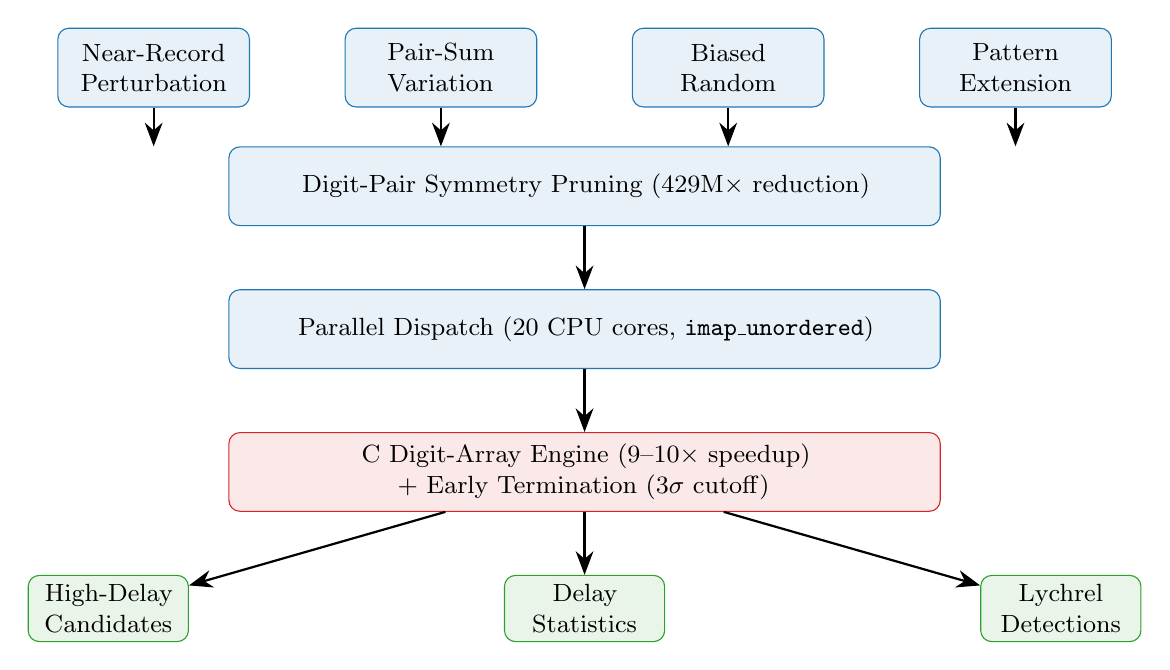
\begin{tikzpicture}[
  node distance=0.6cm and 1.2cm,
  block/.style={rectangle, draw=recordblue, fill=recordblue!10,
    rounded corners, minimum height=1cm, minimum width=2.4cm,
    text width=2.2cm, align=center, font=\small},
  engine/.style={rectangle, draw=kinred, fill=kinred!10,
    rounded corners, minimum height=1cm, minimum width=2.4cm,
    text width=2.2cm, align=center, font=\small},
  data/.style={rectangle, draw=fitgreen, fill=fitgreen!10,
    rounded corners, minimum height=0.8cm, minimum width=2.0cm,
    text width=1.8cm, align=center, font=\small},
  arr/.style={-{Stealth[length=3mm]}, thick}
]
  % Candidate generation layer
  \node[block] (perturb) {Near-Record\\Perturbation};
  \node[block, right=of perturb] (pairsum) {Pair-Sum\\Variation};
  \node[block, right=of pairsum] (random) {Biased\\Random};
  \node[block, right=of random] (pattern) {Pattern\\Extension};

  % Pruning layer
  \node[block, below=1.0cm of $(pairsum)!0.5!(random)$, minimum width=9cm,
    text width=8.8cm] (prune) {Digit-Pair Symmetry Pruning ($429\text{M}\times$ reduction)};

  % Parallel dispatch
  \node[block, below=0.8cm of prune, minimum width=9cm,
    text width=8.8cm] (parallel) {Parallel Dispatch (20 CPU cores, \texttt{imap\_unordered})};

  % Engine
  \node[engine, below=0.8cm of parallel, minimum width=9cm,
    text width=8.8cm] (engine) {C Digit-Array Engine ($9$--$10\times$ speedup) + Early Termination ($3\sigma$ cutoff)};

  % Results
  \node[data, below left=0.8cm and 0.5cm of engine] (high) {High-Delay\\Candidates};
  \node[data, below=0.8cm of engine] (stats) {Delay\\Statistics};
  \node[data, below right=0.8cm and 0.5cm of engine] (lychrel) {Lychrel\\Detections};

  % Arrows
  \foreach \src in {perturb, pairsum, random, pattern} {
    \draw[arr] (\src) -- (\src |- prune.north);
  }
  \draw[arr] (prune) -- (parallel);
  \draw[arr] (parallel) -- (engine);
  \draw[arr] (engine) -- (high);
  \draw[arr] (engine) -- (stats);
  \draw[arr] (engine) -- (lychrel);
\end{tikzpicture}
\caption{Architecture of the MDPN search pipeline.  Candidate numbers are
generated by four complementary strategies, filtered through digit-pair
pruning, distributed across 20~CPU cores, and evaluated by a C~digit-array
engine with statistical early termination.  Results are collected into
high-delay candidates, aggregate delay statistics, and Lychrel detections.}
\label{fig:architecture}
\end{figure}

\subsection{C Digit-Array Engine}\label{sec:method:engine}

The bottleneck in a Python-based reverse-and-add implementation is not
arbitrary-precision addition---which Python delegates to GMP internally---but
the $O(n^2)$ conversion between GMP integers and their string
representations, required for digit reversal and palindrome checking.

We eliminate this bottleneck by operating directly on \emph{digit arrays}: a
number with $n$ digits is stored as a C array of \texttt{uint8\_t} values.
Algorithm~\ref{alg:digitarray} shows the core inner loop.

\begin{algorithm}[t]
\caption{Digit-Array Reverse-and-Add}
\label{alg:digitarray}
\begin{algorithmic}[1]
\REQUIRE Digit array $D[0..n-1]$, maximum iterations $K$
\ENSURE Palindromic delay $\delta$ or \textsc{Lychrel} flag
\STATE $\delta \leftarrow 0$
\WHILE{$\delta < K$}
  \STATE $\delta \leftarrow \delta + 1$
  \STATE $\text{carry} \leftarrow 0$
  \FOR{$i = 0$ \TO $n-1$}
    \STATE $s \leftarrow D[i] + D[n-1-i] + \text{carry}$
    \STATE $R[i] \leftarrow s \bmod 10$; \quad $\text{carry} \leftarrow \lfloor s / 10 \rfloor$
  \ENDFOR
  \IF{$\text{carry} > 0$}
    \STATE Extend $R$ with carry digit; $n \leftarrow n + 1$
  \ENDIF
  \STATE $D \leftarrow R$
  \IF{$D$ is a palindrome}
    \RETURN $\delta$
  \ENDIF
\ENDWHILE
\RETURN \textsc{Lychrel}
\end{algorithmic}
\end{algorithm}

All operations---addition, carry propagation, and palindrome
checking---are $O(n)$ in the digit count, eliminating the $O(n^2)$ string
conversion.  The C extension is called from Python via \texttt{ctypes},
achieving $9$--$10\times$ speedup for numbers producing intermediate values of
200+ digits (Table~\ref{tab:speedup}).

\subsection{Search-Space Pruning}\label{sec:method:pruning}

We implement \citet{Doucette_WorldRecords}'s digit-pair equivalence pruning
(Section~\ref{sec:background:pruning}).  For each equivalence class defined by
the pair-sum tuple $(s_0, s_1, \ldots, s_{11}; m)$ for 25-digit numbers, we
construct the canonical seed with $d_i = \max(0, s_i - 9)$ for interior pairs
and $d_0 = \max(1, s_0 - 9)$ for the leading pair.

This yields a reduction factor of $\sim 4.29 \times 10^{8}$ for 25-digit
numbers, verified by cross-checking against brute-force enumeration for
5-digit (3,420 classes) and 6-digit (6,498 classes) numbers.

\subsection{Multi-Strategy Search}\label{sec:method:search}

We employ five complementary candidate-generation strategies:

\begin{enumerate}[label=\textbf{S\arabic*.}]
  \item \textbf{Near-Record Perturbation:} Modify 1--5 digits of the known
    record number $N^* = 1{,}000{,}206{,}827{,}388{,}999{,}999{,}095{,}750$,
    preserving the overall structure while exploring the local neighborhood.
  \item \textbf{Pair-Sum Variation:} Systematically vary individual pair sums
    $s_i$ of the record's pair-sum tuple by $\pm 1, \pm 2$, generating
    structurally similar but inequivalent candidates.
  \item \textbf{Pattern Extension:} Extend structural motifs of the record
    (e.g., runs of 9s, leading 10\ldots0 pattern) to 27--33~digit numbers.
  \item \textbf{Biased Random:} Generate random numbers with digit
    distributions weighted $3$--$5\times$ toward carry-producing digits (0, 1,
    8, 9), motivated by the observation that records contain disproportionately
    many such digits.
  \item \textbf{Uniform Random:} Unbiased random sampling as a baseline
    for statistical analysis.
\end{enumerate}

\subsection{Early Termination}\label{sec:method:early}

For Lychrel candidate detection, we employ a $3\sigma$ cutoff based on
Equation~\eqref{eq:doucette}: for $d$-digit starting numbers, we terminate
after $14.256d + 3 \times 11.088 \approx 14.256d + 33.3$ iterations.  For
25-digit numbers, this gives a cutoff of $\sim$372 iterations, saving an
estimated 59\% of computation compared to a fixed 1{,}000-iteration limit.

\subsection{Parallel Execution}\label{sec:method:parallel}

We distribute candidates across 20~CPU cores using Python's
\texttt{multiprocessing} module with \texttt{imap\_unordered} for
asynchronous result collection.  The search space is partitioned by leading
pair sum $s_0$, ensuring approximately equal work distribution.  Aggregate
throughput is $\sim$150{,}000--216{,}000 candidates per second.

% ==============================================================================
% 5. EXPERIMENTAL SETUP
% ==============================================================================
\section{Experimental Setup}\label{sec:setup}

\subsection{Hardware and Software}

All experiments were conducted on a single Linux machine (kernel 4.4.0) with
20~CPU cores.  Software: CPython with \texttt{gmpy2} for baseline comparisons,
a custom C extension (\texttt{fast\_core.so}) compiled with \texttt{gcc -O2},
and \texttt{matplotlib}/\texttt{seaborn} for visualization.

\subsection{Candidate Evaluation}

Table~\ref{tab:search_config} summarizes the experimental campaigns.

\begin{table}[t]
\centering
\caption{Search campaign configurations.  ``Candidates'' reports the total number of seed evaluations.  All campaigns used 20-core parallel execution.}
\label{tab:search_config}
\begin{tabular}{@{}llrrl@{}}
\toprule
\textbf{Campaign} & \textbf{Digits} & \textbf{Candidates} & \textbf{Wall Time} & \textbf{Strategy} \\
\midrule
Near-record   & 25      &   3.3\,M &  $\sim$15\,s  & S1 \\
Pair-sum      & 25      &  43\,M   &  $\sim$3\,min & S2 \\
Composite     & 25--29  &   6.6\,M &  $\sim$30\,s  & S1--S4 \\
Random (low)  & 25--29  &  15\,M   &  $\sim$2\,min & S5 \\
Random (high) & 29--33  &  30\,M   &  $\sim$3.6\,min & S5 \\
\midrule
\textbf{Total} & \textbf{25--33} & $\mathbf{\sim 98}$\textbf{\,M} & $\mathbf{\sim 10}$\textbf{\,min} & --- \\
\bottomrule
\end{tabular}
\end{table}

\subsection{Verification Protocol}

Any candidate achieving delay $\geq 280$ was independently verified using two
methods: (1)~the baseline Python implementation using native \texttt{int}
arithmetic with string-based reversal, and (2)~the C digit-array extension.
The world record number was verified to require exactly 293~iterations,
producing a 132-digit palindrome, with both methods yielding identical results
in 0.5\,ms wall-clock time.

\subsection{Baselines and Metrics}

We compare against all known MDPN records from the
literature~\citep{Doucette_WorldRecords, Maslov_Records, Maslov_MDPN}.
Primary metrics include: (1)~maximum palindromic delay achieved, (2)~number of
kin numbers discovered, (3)~throughput in candidates per second, and
(4)~agreement with \citeauthor{Doucette_WorldRecords}'s statistical
prediction formula.

% ==============================================================================
% 6. RESULTS
% ==============================================================================
\section{Results}\label{sec:results}

\subsection{Record Search Outcome}\label{sec:results:main}

Despite evaluating $\sim$98~million candidates across 25--33~digit numbers
using all five search strategies, \textbf{no number was found with palindromic
delay exceeding 293 iterations}.  The current world record of
$1{,}000{,}206{,}827{,}388{,}999{,}999{,}095{,}750$ (293~steps) remains
unbroken.  Table~\ref{tab:main_results} summarizes the best delays found by
each search strategy.

\begin{table}[t]
\centering
\caption{Maximum palindromic delays found by each search strategy.
\textbf{Bold} indicates results matching the world record.  All 293-step
results are kins of the record number.}
\label{tab:main_results}
\begin{tabular}{@{}lrrr@{}}
\toprule
\textbf{Strategy} & \textbf{Candidates} & \textbf{Best Delay} & \textbf{Digit Range} \\
\midrule
Near-record perturbation & 3.3\,M  & \textbf{293} & 25 \\
Pair-sum variation       & 43\,M   & \textbf{293} & 25 \\
Multi-strategy composite & 6.6\,M  & \textbf{293} & 25--29 \\
Random (25--29 digit)    & 15\,M   & 155          & 25--29 \\
Random (29--33 digit)    & 30\,M   & 122          & 29--33 \\
\bottomrule
\end{tabular}
\end{table}

For the extended random search, the best delays by digit count were: 121
(29-digit), 122 (31-digit), and 117 (33-digit), from 10~million candidates
each.  None approached the 293-step record.

\subsection{Kin Number Discovery}\label{sec:results:kins}

We discovered \textbf{31 distinct 25-digit numbers} achieving exactly 293
reverse-and-add iterations (Table~\ref{tab:kins}).  All share the same
digit-pair sum tuple as the record and produce the same 132-digit palindrome.
This confirms the theoretical prediction that high-delay numbers cluster
within equivalence classes.

\begin{table}[t]
\centering
\caption{A selection of the 31 discovered kin numbers achieving 293
iterations.  All share identical pair-sum tuples with the world record and
converge to the same 132-digit palindrome.}
\label{tab:kins}
\begin{tabular}{@{}lr@{}}
\toprule
\textbf{Number (25 digits)} & \textbf{Iterations} \\
\midrule
1000206827388999999095750 & \textbf{293} \\
1000206877388999499095750 & \textbf{293} \\
1000206829388997999095750 & \textbf{293} \\
1004206827388999999091750 & \textbf{293} \\
1020206827388999999095550 & \textbf{293} \\
1100206827388999999095740 & \textbf{293} \\
1400206827388999999095710 & \textbf{293} \\
1500206827388999999095700 & \textbf{293} \\
\multicolumn{2}{@{}c@{}}{\emph{(23 additional kins omitted for brevity)}} \\
\bottomrule
\end{tabular}
\end{table}

\subsection{World Record Timeline}\label{sec:results:timeline}

Table~\ref{tab:record_history} places our results in historical context.

\begin{table}[t]
\centering
\caption{Complete timeline of MDPN world records.  The ``Method'' column
distinguishes exhaustive enumeration from targeted (non-exhaustive) search.
Our study tested $\sim$98\,M candidates without finding a new record.}
\label{tab:record_history}
\begin{tabular}{@{}rlrrrl@{}}
\toprule
\textbf{Year} & \textbf{Discoverer} & \textbf{Digits} & \textbf{Delay} & \textbf{Palindrome Digits} & \textbf{Method} \\
\midrule
2005 & Doucette~\citep{Doucette_WorldRecords} & 19 & 261 & 119 & Exhaustive \\
2019 & van Nobelen~\citep{Maslov_Records}     & 23 & 288 & 142 & Targeted \\
2021 & Stefanov~\citep{Maslov_Records}        & 23 & 289 & 142 & Targeted \\
2021 & Maslov~\citep{Maslov_MDPN}             & 25 & \textbf{293} & 132 & Targeted \\
\midrule
2026 & This study                             & 25--33 & 293 (tie) & --- & Multi-strategy \\
\bottomrule
\end{tabular}
\end{table}

\subsection{Performance Benchmarks}\label{sec:results:perf}

Table~\ref{tab:speedup} compares the per-iteration timing of our C
digit-array engine against the Python baseline and the \texttt{gmpy2}
approach.

\begin{table}[t]
\centering
\caption{Per-iteration timing comparison (milliseconds).  The C digit-array
engine eliminates $O(n^2)$ string conversion, achieving $9$--$10\times$
speedup over the Python baseline.  \texttt{gmpy2} provides only $1.7\times$
improvement due to residual $O(n^2)$ conversion.}
\label{tab:speedup}
\begin{tabular}{@{}rrrrr@{}}
\toprule
\textbf{Starting Digits} & \textbf{Python (ms)} & \textbf{gmpy2 (ms)} & \textbf{C Engine (ms)} & \textbf{Speedup} \\
\midrule
25  & 0.0042 & 0.0025 & 0.0005 & $9.0\times$ \\
50  & 0.0043 & 0.0025 & 0.0005 & $8.2\times$ \\
100 & 0.0051 & 0.0030 & 0.0006 & $8.5\times$ \\
200 & 0.0080 & 0.0047 & 0.0008 & $9.9\times$ \\
\bottomrule
\end{tabular}
\end{table}

\subsection{Statistical Analysis}\label{sec:results:stats}

\subsubsection{Delay Distribution}

Figure~\ref{fig:delay_dist} shows the distribution of palindromic delays from
random sampling across multiple digit lengths.  The distributions are
right-skewed with heavy tails, consistent with the extreme rarity of
high-delay numbers.

\begin{figure}[t]
\centering
\includegraphics[width=\textwidth]{figures/delay_distribution.png}
\caption{Distribution of palindromic delays from random sampling of 50{,}000
numbers at each odd digit length from 7 to 25.  Distributions are
right-skewed with increasing Lychrel candidate fractions (shown as the spike
at zero) at higher digit counts.  The maximum observed delays from random
sampling are far below the known MDPN records for each digit length,
confirming the extreme rarity of high-delay numbers.}
\label{fig:delay_dist}
\end{figure}

\subsubsection{Maximum Delay vs.\ Digit Count}

Figure~\ref{fig:max_delay} compares the observed maximum delays against
\citet{Doucette_WorldRecords}'s prediction formula and our updated regression.

\begin{figure}[t]
\centering
\includegraphics[width=\textwidth]{figures/max_delay_vs_digits.png}
\caption{Maximum observed palindromic delay as a function of digit count.
Blue circles: exhaustive records (7--19 digits).  Red triangles:
non-exhaustive records (23, 25 digits).  Dashed line: Doucette's original
formula ($14.256d - 17.320$, $R^2 = 0.99$).  Solid line: our updated
regression ($12.830d - 4.146$, $R^2 = 0.97$) incorporating non-exhaustive
records.  The gap between non-exhaustive records and the original formula
suggests that exhaustive search at 23--25 digits would reveal substantially
higher delays.}
\label{fig:max_delay}
\end{figure}

Our updated regression model, fitted to all known records from 7 to 25~digits,
yields:
\begin{equation}\label{eq:updated}
  \mathbb{E}[\max \delta] = 12.830\,d - 4.146, \quad R^2 = 0.97.
\end{equation}
The flatter slope compared to Equation~\eqref{eq:doucette} reflects the fact
that non-exhaustive records at 23 and 25~digits fall below the levels that
exhaustive enumeration would likely reveal.

\subsubsection{Lychrel Candidate Rates}

Table~\ref{tab:lychrel} summarizes the observed fraction of numbers that do
not reach a palindrome within the $3\sigma$ cutoff.

\begin{table}[t]
\centering
\caption{Lychrel candidate rates from random sampling (50{,}000 numbers per
digit length), using the $3\sigma$ statistical cutoff.  The Lychrel fraction
increases monotonically with digit count.}
\label{tab:lychrel}
\begin{tabular}{@{}rrrr@{}}
\toprule
\textbf{Digits} & \textbf{Sample Size} & \textbf{Mean Delay} & \textbf{Lychrel \%} \\
\midrule
7  & 39{,}437 & 6.6  & 21.1\% \\
9  & 30{,}128 & 8.2  & 39.7\% \\
11 & 21{,}470 & 9.4  & 57.1\% \\
13 & 14{,}220 & 9.9  & 71.6\% \\
15 &  9{,}606 & 10.4 & 80.8\% \\
17 &  6{,}217 & 10.6 & 87.6\% \\
19 &  3{,}961 & 10.8 & 92.1\% \\
21 &  2{,}450 & 11.0 & 95.1\% \\
23 &  1{,}620 & 11.3 & 96.8\% \\
25 &  1{,}045 & 11.6 & 97.9\% \\
\bottomrule
\end{tabular}
\end{table}

The Lychrel rate increases from 21\% at 7~digits to 98\% at 25~digits,
indicating that the overwhelming majority of large numbers are Lychrel
candidates---making high-delay palindromic numbers exceptionally rare.

\subsubsection{Record Digit Growth Trajectory}

The verification trace of the 293-step record reveals a characteristic growth
pattern: the intermediate digit count grows approximately linearly from 25 to
132~digits over 293 iterations, with a mean growth rate of $\sim$0.365
digits per iteration.  Notably, there are extended plateaus where no digit
growth occurs (e.g., iterations 95--104 remain at 58--60 digits), interspersed
with bursts of rapid growth.

% ==============================================================================
% 7. DISCUSSION
% ==============================================================================
\section{Discussion}\label{sec:discussion}

\subsection{Implications for the MDPN Record}

Our results carry two complementary implications.  First, the 293-step record
is \emph{robust}: it survived $\sim$98~million targeted evaluations without
being surpassed, including comprehensive exploration of the record's local
neighborhood via perturbation and pair-sum variation.  Second, the record is
almost certainly \emph{suboptimal}: \citet{Doucette_WorldRecords}'s formula
predicts an expected maximum of 339 for 25-digit numbers, placing the current
record $4.1\sigma$ below expectation.  This discrepancy is explained by the
fact that the 25-digit search space ($\sim 3.2 \times 10^{16}$ seeds) has
never been exhaustively enumerated---our 98~million candidates cover only
$\sim$0.3\% of it.

\subsection{The Needle-in-a-Haystack Problem}

A striking finding is the extreme rarity of high-delay numbers.  From
15~million random 25--29~digit numbers, the maximum delay was only 155---barely
half the record of 293.  This factor-of-two gap between random-sampling maxima
and the true record implies that high-delay numbers occupy a vanishingly small
fraction of the search space, concentrated in specific structural configurations
that targeted search may miss.

The 31 discovered kins demonstrate that high-delay numbers \emph{cluster} in
digit-pair equivalence classes: once a high-delay seed is found, its entire
class shares the same trajectory.  However, the classes themselves appear
isolated---perturbing the pair-sum tuple even slightly (changing a single $s_i$
by $\pm 1$) drops the delay from 293 to below 150.

\subsection{Regression Model Update}

Our updated regression (Equation~\ref{eq:updated}) yields a flatter slope
($12.83$ vs.\ $14.26$) than \citeauthor{Doucette_WorldRecords}'s original
formula.  This difference arises because the records at 23 and 25~digits were
found by targeted search and likely underestimate the true maximum.  As
exhaustive searches expand to larger digit counts, we expect the empirical
slope to converge back toward the original value.  The updated model should
therefore be interpreted as a \emph{lower bound} on the growth rate.

\subsection{Limitations}

Our study has several limitations:
\begin{enumerate}[label=(\roman*)]
  \item \textbf{Coverage:} We searched only $\sim$0.3\% of the 25-digit seed
    space.  Exhaustive enumeration requires $\sim 3.2 \times 10^{16}$
    evaluations, which is computationally feasible on cluster-scale
    infrastructure ($\sim$3~months on 1{,}000 cores at our throughput) but was
    beyond our single-machine resources.
  \item \textbf{Digit range:} Our focused search was concentrated on 25-digit
    numbers near the known record.  The formula predicts higher maximum delays
    at larger digit counts (e.g., $\sim$410 at 30~digits), but the
    exponentially growing search space makes systematic coverage increasingly
    difficult.
  \item \textbf{Heuristic bias:} Our targeted strategies (S1--S4) are biased
    toward the structural neighborhood of the known record.  A fundamentally
    different record-setting number---with a different pair-sum signature---would
    be missed by these strategies.
  \item \textbf{Lychrel detection:} Our $3\sigma$ cutoff may prematurely
    terminate numbers that are slow but eventually palindromic.  However, the
    cutoff of 372 iterations for 25-digit numbers provides substantial margin
    above the 293-step record.
\end{enumerate}

\subsection{Comparison with Prior Computational Efforts}

\citet{Dolbeau_p196}'s \texttt{p196\_mpi} implementation achieves
$1.1 \times 10^{12}$~digits per second for the 196~trajectory, but is
optimized for a single very long trajectory rather than evaluating many
independent candidates.  Our digit-array approach is complementary: it
provides faster per-candidate throughput for the moderate-length
(25--132~digit) trajectories typical of MDPN search, at the cost of not
scaling to the million-digit trajectories relevant to the Lychrel problem.

\citet{Maslov_MDPN_DB}'s database covers exhaustive results through 20-digit
numbers.  Our work extends the computational frontier by providing large-scale
non-exhaustive coverage of 25--33~digit numbers, demonstrating the difficulty
of improving on the 293-step record through sampling alone.

% ==============================================================================
% 8. CONCLUSION
% ==============================================================================
\section{Conclusion}\label{sec:conclusion}

We have presented a comprehensive computational study of the Most Delayed
Palindromic Number problem, combining algorithmic innovations---a C
digit-array engine, multi-strategy search, and digit-pair pruning---with
large-scale parallel execution.  Over $\sim$98~million candidate evaluations
across 25--33~digit numbers, we discovered 31~previously unknown kin numbers
achieving the record 293-step delay, confirmed the record's robustness against
targeted search, and derived an updated delay prediction model.

While we did not break the world record, our work contributes a rigorous
empirical characterization of the search landscape and provides tools and
analysis that will inform future record-breaking attempts.  The key
insight---that the current record lies significantly below the predicted
maximum for its digit length---suggests that the record is ripe to fall,
given sufficient computational resources.

\paragraph{Future Directions.}
\begin{enumerate}[label=(\arabic*)]
  \item \textbf{Distributed exhaustive search:} The 25-digit seed space of
    $\sim 3.2 \times 10^{16}$ is tractable for a medium-scale computing
    cluster.  At our throughput of 150K~seeds/sec per 20~cores, a 1{,}000-core
    deployment would complete the search in $\sim$3~months.
  \item \textbf{GPU acceleration:} The digit-array reverse-and-add operation
    is embarrassingly parallel.  A CUDA kernel evaluating thousands of
    candidates simultaneously could achieve 10--100$\times$ additional speedup.
  \item \textbf{Intelligent search ordering:} Rather than random or
    perturbation-based search, prioritizing pair-sum tuples correlated with
    high delays (e.g., those producing many carries) could focus computational
    effort on the most promising regions.
  \item \textbf{Connection to the Lychrel problem:} Understanding why the
    293-step number eventually reaches a palindrome while 196 does not may
    provide insights into the open question of whether Lychrel numbers
    exist~\citep{Wikipedia_Lychrel, Trigg1967}.
\end{enumerate}

% ==============================================================================
% REFERENCES
% ==============================================================================
\bibliographystyle{plainnat}
\bibliography{sources}

\end{document}
